\chapter{Analysis}

\section{Problem Area}
		As this report will try to improve current tools in modern musical education, it is important to understand how the current education functions. This section will take a closer look at the definition of music, why it is important to teach music to students and how it is currently taught.\\
		
	\subsection{What is music? Audiation:}
	\begin{quote}
	\textit{Sound itself is not music. Sound becomes music through audiation, when, as with language, you translate sounds in your mind and give them meaning.}\\
	\end{quote}
	
	Everyone has a meaning about the sound they hear, and the meaning differs from individual to individual. Audiation is the concept of assimilating and comprehending music heard by the individual, either in the present or in the past. We can also audiate through reading notations, composing contemporary music or improvising on an instrument.
	The concept of audiation is similar to the concept of language:\\
	
	\begin{quote}
	\textit{"Consider language, speech and thought. Language is the result of the need to communicate. Speech is the way we communicate. Thought is what we communicate. Music, performance and audiation have parallel meanings. Music is the subject of communication. Performance is the vehicle for communication. Audiation is what is communicated."}\\
    \end{quote}
	
	An individual can begin audiating shortly after hearing music, to give meaning to the sound. What the individual can take from the audiation depends on that particular individuals previous audiation. The concept is similar to regular conversation – if a group of people are talking, each individual will take their own comprehension of the conversation with them. This comprehension is based on existing knowledge and experience on the topic. 
	The concept of audiation increases the chance of remembering what the individual learns long term. Everyone can remember 7 +/- 2 things(REF), however, if the individual tries to remember something without comprehending it, it quickly slips away again. If students have issues with vocal or instrumental techniques, or they struggle with memory lapses, it is most like due to them not auditing while playing or singing. If the student audiates away from their instrument, it can correct techniqual and memory issues, including issues related to tone. Audiating before performing sound is key to learning music. Instruments should not be seen as the tool to learn how to understand music, but rather the tool to express the music:\\
	
	\begin{quote}
	\textit{“Just as a calculator becomes a crutch for students who cannot multiply or divide, so music instruments become crutches for students who cannot audiate. This is immediately obvious when students learn to play scales by memorizing fingerings. Although students may recognize they are performing with poor intonation or inaccurate rhythm, their lack of audiation is virtually impossible for them to correct those problem by themselves. Audiation may be expressed through a music instrument, but it cannot be taken from a music instrument.”}\\
    \end{quote}

	Audiation potential itself cannot be taught but rather depends on how natural musical aptitude comes to the individual. However, while Audition potential cannot be taught, students can be taught how to maximize their music achievement:\\
	
	\begin{quote}
	“By providing children and students with appropriate knowledge and experiences, they can be taught how to audiate, that is, how to use inherent audiation as determined by their music aptitude, to maximize acquired music achievement as determined by the quality of a particular educational environment.”\\
	\end{quote}

	The issues become evident if the students don’t learn audiation, notation and music theory in the proper sequence, they will be unable to make sense and add meaning the sound and music they hear or the notations they read. It is particularly evident with wind instruments Techniques refer to the methods the teacher uses to teach as well as the tools applied to achieve certain goals in different activities.. If the students are unable to tonally audiate what they see in the notations, but still manipulate the keys or valves on the instrument as the notation instructions, the student will often fall out of tune.
	Everyone can learn some degree of music. Similar to how everyone has at least some amount of intelligence, everyone has some amount of music aptitude, so put in other words, everyone is musical. Everyone is capable of learning to listen to and perform music to some extent of success. Generally, two-thirds of humans are average – that includes average music aptitude.
	Also it is important to get students of to a good start. The foundation that is created in the early ages is a substantial influence on the music achievement of the student. Most likely, the guidance received in the early stages of their musical careers is a bigger influence, than the guidance the students receive in the higher grades or at colleges and universities. If the students musical skillset is not properly maintained, they will severely decrease over time.
	In order to maintain the skillset properly, the techniques used by teachers have to be considered as
	they are highly important. When it comes to tonation, the rhythm patterns and harmonic patterns are the most prevalent materials and they’ve remained similar for a long time across different nationalities and cultures as they belong to the basics of audiation. On the opposite site, we have activites that include larger classrooms. These will vary a lot depending on the culture, age and experience.\\
	
	
	\subsection{Why learn music? The impact of musical education}
	Several studies have shown that different types of musical engagement in a variety of ways over a lifespan has an impact on several aspects of personal growth and development. As concluded in the article "The power of music: Its impact on the intellectual, social and personal development of children and young people":\\
	
	\begin{quote}
		\textit{"This overview provides a strong case for the benefits of active engagement with music throughout the lifespan"}\cite{powerOfMusic}\label{quote:powerOfMusic}.\\
	\end{quote}
	
	Linguistic abilities and musical training seems to be linked, due to shared brain mechanisms being used to process music and language. Precision in the perception of speech related contrasts, in pitch patterns and other distinctive speech elements have been reported to be associated with musical ability\cite{languageSkills}.\\
	
	A study focused on literary skills showed that a group of second grade students(n = 47) taking piano lessons over a 3-year period had significantly better vocabulary and verbal abilities than a group of control students(n = 57) that did not receive music lessons\cite{vocabularySkills}.\\
	
	Some aspects of mathematical skills have also been shown to be improved by musical training. For example the subdivision process required to read and play from music scores in order to play and keep a rhythm\cite{powerOfMusic}.\\
	
	Other abilities have also been reported to be affected by musical training such as creativity, social and personal development, physical development, health and wellbeing\cite{powerOfMusic}.\\
	
	According to the article \textit{Interactive music video games and children's musical development} there are 5 basic music elements that should be learned in order to get a good understanding and appreciation of music\cite[p.~99]{interactiveMusicVideoGames}:
	\begin{itemize}\label{list:basicMusic}
		\item Duration
		\item Pitch
		\item Tone color
		\item Dynamics
		\item Structure\\
	\end{itemize}
	
	In another study, which focused on integration of music in the elementary classroom, results were positive. Musical activities activate both the analytical and creative side of the brain, and learning other subjects becomes easier with the addition of a musical element, as the speed at which information is processed increases. An example of this is learning the math of money exchange through music note denotations\cite{musicIntegration}.\\
	
	Through the initial research, it can be assumed that musical education is important for the development of young students in many facets of life. In order to consider if certain tools can improve the current musical education, an analysis of the study plan applied to the education of elementary school students across Denmark will be analysed.
	
	\subsection{How is music taught? The Study plan}
	
	According to the study plan, the children are required to learn three basic teaching elements. Within these are musical performance, musical creation and musical understanding.
	
	\subsection*{Musical performance}
	Musical performance includes teachings about singing, movement and playing instruments. More specifically teaching the children about how to sing individually and in groups, as well as teaching them about different kinds of singing and songs. Furthermore, teaching the children about movement in a musical context, such as dancing and rhythmic movement. Finally, being able to play the basics of different instruments, such as drums, guitar, piano or keyboard and different wind instruments.
	
	\subsection*{Musical Creation}
	Musical creation includes the teachings of different abilities in relation to create, alternate or improvise musical pieces. The children should be able to compose music with the ability to remember time and tempo when creating music. Furthermore, the children should be able to form and shape sound into something rhythmic. Besides creating music, the children should also be able to change music with the help of adding sounds, or changing the pitch or pace of sound. Finally, the children should be able to improvise music without being given a specific assignment to follow.
	
	\subsection*{Musical Understanding}
	Musical understanding is, first of, to be able to express music in other forms than sound. For an example, they should be able to express themselves verbally about music and be able to draw music. The children should have knowledge about instruments, and the ability to distinguish the different instruments from their appearance as well as their sound. The children should be able recognize specific elements in a musical piece and identify them. Finally, they should have the knowledge of musical history, in relation to different music genres as well as music from different time periods.
	\\
	
	When the children get older, they will be introduced to digital tools and synthesizers to be used in the classroom. These tools might include iPad or Garageband. On these devices, they are asked to compose a musical piece using the aforementioned knowledge.\\
	In the lower grades, the children are working more with analog instruments as well as singing to develop a musical foundation for their education.
	\\
	
	The study plan opens for a broad interpretation of elements that are taught and with which tools this knowledge gets taught. After analyzing the study plan, it became evident that an interview with a teacher is necessary to get a profound understanding of how the course “Music” is taught in elementary schools.\\
	
	\subsection{Interview with Hanna Jørgensen}
	Hanna Jørgensen is a teacher in music at both elementary school level and Danish Gymnasium level at “Sankt Annæ Skole”. She is also a pedagogue in Musical Pedagogy at the National Music Conservatory. Besides the aforementioned credentials, she is also involved in “Børne og Ungdoms Forvaltningen”, which is an organization that tries to improve the quality of life among children and young people. She is interviewed to help establish a detailed view on how the current musical education functions, and to help locate issues within the musical curriculum for elementary school children.\\
	
	ANALYSE INTERVIEW HERE\\
	
	SUB CONCLUSION (leading into analysis) HERE\\
\section{Learning}
	\subsection{Learning Defined}\label{sec:learning}
	Learning is the process described as obtaining or modifying knowledge. The ability to learn exists for most living things i.e humans, animals, plants and some machines. \\
	\\
	There are many types of learning, this report will mainly focus on Active Learning and Passive Learning due to being the main types of learning, when talking about education.
	
	\subsection*{Active Learning}
	Active learning comes from a person taking control of their own learning experience. If a student just sits and listens, they will not achieve as much of their learning experience as possible. Active learning comes to play, when the student actively does more than listen. They read, write discuss and engages themsevles at the given topic. This also includes doing excersices and solving topic specific problems\cite{activelearning}. The use of active learning in a classroom is vital to improve the learning experience of the students. Furthermore, when not using active learning, up till 70\% of the obtained knowledge is lost within the next 24 hours \cite{learning}.\\
	
	The retention of learning is the concept describing the processed information travelling from the short term memory to the long term memory. Furthermore, retention of learning describes how processed information can be forgotten. As aforementioned attending a lecture without actively participating except listening, can cause a person to lose the majority of information obtained withing 24 hours. Multiple theories within the retention of learning also suggests that the information is not lost, but a person is just unable to recall the information \cite{retention}.
	In figure \ref{fig:activelearn} the concept of retention of learning is displayed. The figure displays how different ways of learning affects the amount of information learned and remembered. In the bottom bracket, there is the lectures, reading and audiovisual elements. These are the elements which does not actively include the student when obtaining the information, and is therefore the least effective way of learning. In the middle bracket, demonstration, discussion, exercises and play is displayed, these elements provides a hands-on approach to learning and increases the amount of information obtained significantly. This means interaction and taking an active part in solving a problem, will increase the chance of remembering information about the topic. In the top bracket, there is the "learning by doing", aspect containing; working with a coach and practicing is displayed. These aspects are likely to provide the best results. This is because there is a personal approach and the motivation by the student is higher at this point\cite{retention}. 
	
		\begin{figure}[H]
			\centering
			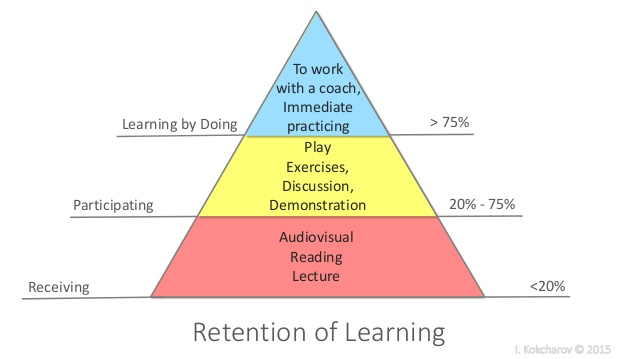
\includegraphics[width=0.9\linewidth]{figure/Analysis/skillslearn}
			\caption{Retention of Learning, taken from \href{https://www.slideshare.net/igorkokcharov/kokcharov-skillpyramid2015}{\color{blue}here}}
			\label{fig:activelearn}
		\end{figure}
	\todo{Instead of "here" in the caption, we need to add a name, author, webpage or something}
	
\subsection*{Passive Learning}
sed where the students are not getting involved in the lecture. This form of teaching is usually seen on universities where the professors gives a lecture, and does not provide assignments or feedback to the students. This means that the learning method belongs in the bottom bracket of the retention of learning triangle as seen above. This way of teaching is usually the least efficient when the goal is to teach or alter information.\\
	\\
	\subsection*{Sub Conclusion}
	When learning is the goal in an education enveironment, both active learning and passive learning are being utilized. Based on the findings, active learning will provide a better learning experience where the student will be able to remember more information if done correct. This means that participation and practice as well as motiation and interaction are essential to optimise the learning experience the most.
	   
	\subsection{Collaborative learning}
	
	Associate professor from Aarhus University School of Business and social sciences writes in his book, \textit{Læring i praksis}(Learning in practice):
	
	\begin{quote}
		"\textit{The learning process is social as we humans are created as pack animals that learn with each other and from each other}"\footnote{Danish translation: "Læreprocessen er social for vi mennesker er skabt som flokdyr, der lærer med hinanden og af hinanden"}\cite[p.~17]{laeringIPraksis}
	\end{quote}

	This subsection explores learning in a collaborative perspective and what the potential benefits are of implementing this approach in music education and in general.\\
	
	There has been a lot of research on collaborative learning in various educational contexts. However, the more artistic educations, like music, have been slightly overlooked\cite{collaborativeLearningTeachers}\cite{collaborativeMusicAnalysis}\cite{collaborativeLearningReview}.
	The article \textit{The Experiences of Elementary Music Teachers in a Collaborative Teacher Study Group} states, based on research outside of a musical context, that:\\
	\begin{quote}
		\textit{"collaboration can improve learning outcomes if students make a conscious effort to coordinate their efforts and are able to come to a shared conceptual understanding of the problem being solved"}\cite{collaborativeLearningTeachers}.\\
	\end{quote}
	
	However, it is not an entirely unexplored area, and studies have shown that musical collaboration stimulates students critical and creative thinking, and rich musical experiences can surface from combining ideas from larger groups\cite{collaborativeLearningTeachers}. 
	The article introduces three principles of collaboration, that are based on interviews with three teachers:\\
	\begin{enumerate}
		\item Collaboration facilitates student self-expression and independence.
		\item Students who are collaborating share goals. The teacher allows space for or guides students in creating productive student-student interactions.
		\item A teacher collaborating with her students facilitates their movement toward a shared goal. Teacher provides necessary background skills, creates student buy-in for the goal, and then fades away to allow students to take ownership.\\
	\end{enumerate}
	
	The first principle is at work when students, for example, are divided into smaller groups, and find themselves focusing on a task that generates communication, arguments and discussions without the teachers involvement. They will show independence as they, for example, individually will try to convince others to reach the same conclusions. Through this type of work a student can develop skills in dialog, negotiation and compromise that are also useful later in life as the students grow up and get jobs of various kind\cite{collaborativeLearningReview}\\
	
	The second principle is related to a student groups shared motivation while focusing on a shared goal, for example presenting their work for the entire class, and sharing the responsibility to reach that goal.\\
	
	The third principle is related to the second principle and involves the teacher in a teacher-student collaboration that also can be present withing the classroom. Here the teacher will for example instruct the student with harmonies, rhythms, chord progressions etc. after which the teacher gradually removes him/herself and let the students take control over the task at hand and their shared goal.\\
	
	Collaborative learning outside of music is about constructing a pool of shared knowledge, breaking down cultural barriers and also uniting students and teachers in a pursuit of knowledge building. Within music education it also expands the field of influence while building social relations\cite{collaborativeLearningReview}.
	
	\subsection*{Sub conclusion}
	Collaborative learning has an impact on various aspects of personal development. It has a positive impact on creativity, musical influence and social interactions that could potentially be very useful later in life.
	

	\subsection{Interaction in a learning perspective}
	As mentioned in chapter \ref{sec:learning} a hands-on approach and interaction is important to get an efficient learning experience. This chapter will focus and go in depth interaction in correlation to learning.
	
	First of, interaction is the description of the occurrence when objects interacts with each other, this can be a person interacting with an object, or an object interacting with another object etc.
	
When trying to understand music in an interactive sense, one might look at another medium that incorporates interactivity: video games. In particular, one could look at interactive video games that focuses on playing or teaching music. Lily Gower and Janet McDowall conducted a study, in 2012, centered around the educational qualities gained from playing such interactive music video games\cite{interactiveMusicVideoGames}. The study aimed to establish if interactive music video games had an educational value when integrated into the existing music education.\\

The different games mentioned in the study were Guitar hero (See \autoref{sec:guitarHero}), SingStar and Wii Music. What these games have in common is that they all use interactivity as a means to playing music, be it with a guitar shaped controller, a microphone or the Wii remote held like an instrument. These games try to emulate what it would \textit{feel like} to play a guitar, sing or play different instruments.\\

The study interviewed two music teachers of different musical abilities, and 9 music students aged 11-14 (5 male and 4 female) from different socio-economic situations. The student participants came into the study with different levels of musical experience. The interviews were semi-structured of nature to allow free flowing conversation. Interviews with the children participants revolved around their prior music backgrounds and past experiences with interactive music video games. The interviews with the teacher participants discussed their personal views and experiences with interactive music video games, like Guitar hero (\autoref{sec:guitarHero}), in relation to music education.\\

Teacher two said during the interview that:
\begin{quote}
	\textit{"...the whole debate about whether it’s music making, that’s a whole other debate, but whether it’s developing some across the board generic skills, I’d say yes."}\cite[p.~98]{interactiveMusicVideoGames}.\\
\end{quote}
\todo{sddffsfsd }
Meaning a belief in interactive music video games giving the students some educational values in a more general music setting. In addition, when asked about coordination benefits, Teacher two said the following:
\begin{quote}
	\textit{"...To play at the higher levels of that game [Guitar Hero] requires very high level coordination skills and you’re coordinating visually with what you’re playing as an instrument. So it’s not so different I think physiologically from what a musician does anyway which is to respond to a conductor visually, respond to the music score visually, and then play accordingly to a set tempo, and timing is everything. So, the game is about scoring high scores all based on your capacity to play in time on the right note and what’s that sound like? Sounds like music playing to me."}\cite[p.~98]{interactiveMusicVideoGames}.\\
\end{quote}
Teacher two has a firm belief that Guitar hero specifically has a high coordination requirement, and thus to play at the higher difficulty levels of the game, you need good eye-hand coordination, which he thinks correlates in a physiological way directly to the way real music is played.\\

When the student participants where asked about their musical knowledge gained from playing interactive music video games, one girl said:
\begin{quote}
	\textit{"Yeah, so it’s like you find out about more songs that you don’t know about . . . there’s a lot of songs that you don’t know about and then you like listen to them and then you get into either like the artist or the type of songs or you just listen to that song and stuff and then you go looking on the net for other songs of that type and stuff, so it opens up a whole lot of stuff."}\cite[p.~100]{interactiveMusicVideoGames}.\\
\end{quote}	
The participant felt that she had gained music knowledge, and broadened her musical identity. The exposure to the new music, gave her an interest in new artists and genres she might not have known about.\\

The discussion about whether or not interactive music video games provide the children with a basic understanding of essential musical elements, is argued by Lily Gower and Janet McDowalls, to be that they at least learned about pitch and rhythm, while maybe not the rest of the five elements seen in \autoref{list:basicMusic}. Meaning the interactive music video games assisted the children in Lily Gower and Janet McDowall's study develop some basic music skills, that might correlate to real music making\cite[p.~99]{interactiveMusicVideoGames}, and potentially could assist other children in similar age groups.

\subsubsection*{Sub conclusion}
In conclusion, the children in the study\cite{interactiveMusicVideoGames} did seem to learn at least two basic musical elements from interactive music video games, being pitch and rhythm. In addition the children also felt they had gained musical knowledge from these games. Hence interactivity in musical education, it being from Guitar Hero, SingStar or another interactive music medium, seems to assist children in development of some aspects of musical abilities.

\section{Motivation theory}
Motivation is an integral part to learning\cite{motivationGameDesign}, and is therefore important when looking at ways to assist children in learning music. The most fundamental motivational theory is the one called Self determination theory (SDT)\cite{SDT}. SDT proposes that motivation is divided into two brackets; Intrinsic motivation and extrinsic motivation\cite{SDT}. 

\subsection*{Intrinsic motivation} 
	This the inherent need humans have to learn, explore and widen their knowledge\cite{SDT}. It also is also the motivation behind doing tasks without having any rewards or benefits associated directly with that task\cite{SDT}. To establish what influences intrinsic motivation, the study behind SDT\cite{SDT}, created Cognitive evaluation theory(CET) as subtheory within the existing SDT. CET is the theory that focuses on competence and autonomy in relation to intrinsic motivation. The first part of the theory is that social-contextual events that improve the feeling of competence according to the performed action\cite[p.~70]{SDT}. These social-contextual events might include rewards, feedback and communications\cite[p.~70]{SDT}. For intrinsic motivation to be improved, the action that is performed must be felt as though it was by the person's own desire. The feeling of competence must be accompanied by a feeling of autonomy, else intrinsic motivation will not be improved\cite[p.~70]{SDT}.\\

\subsection*{Extrinsic motivation}
	Extrinsic motivation is the motivation that drives a person, depending on a reward associated with performed action. From the SDT theory extrinsic motivation is defined as: 
	\begin{quote}
		\textit{The term extrinsic motivation refers to the performance of an activity in order to attain some separable outcome and, thus, contrasts with intrinsic motivation, which refers to doing an activity for the inherent satisfaction of the activity itself.}\cite[p.~71]{SDT}.\\
	\end{quote}
	Internalization and integration in extrinsic motivation.\todo{Flesh this out.}

\begin{itemize}
	\item[ ] \textbf{Intrinsic motivation} pushes us to act freely, on our own, for the sake of it.\\
	\item[ ] \textbf{Extrinsic motivation} pulls us to act due to factors that are external to the activity itself, like reward or threat.\\
	\item[] \textbf{Amotivation} denotes the absence of motivation.\\
\end{itemize}

\begin{figure}[H]
	\centering
	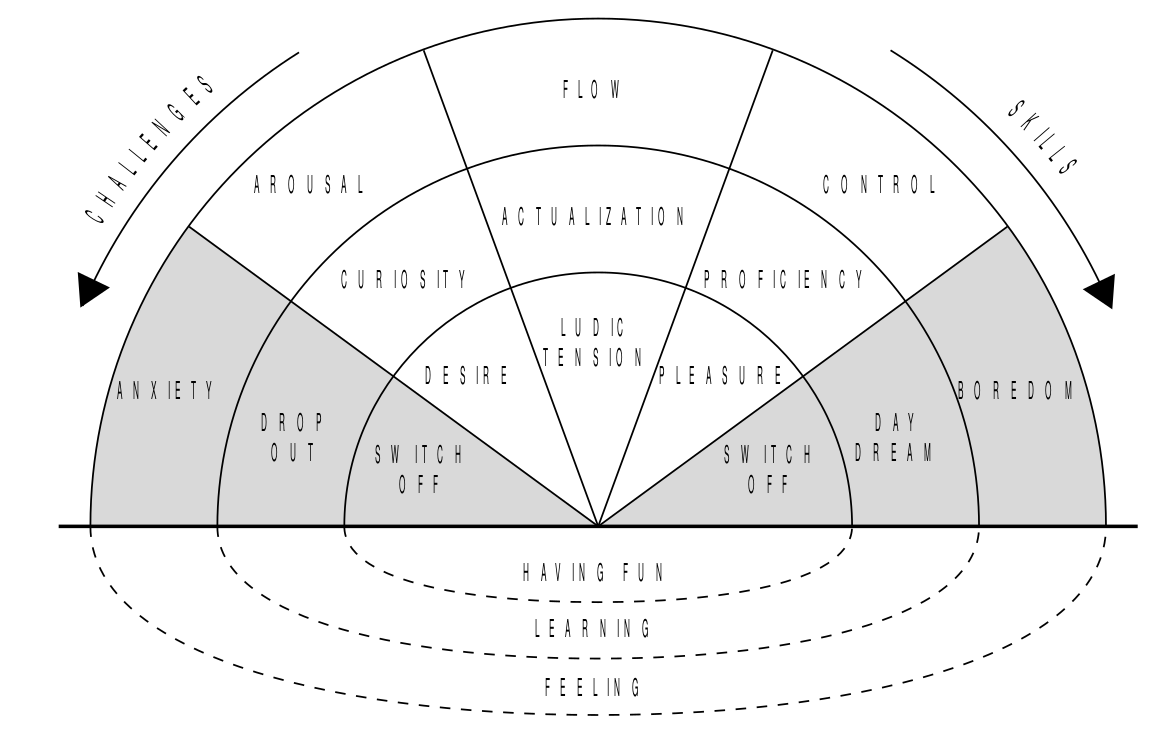
\includegraphics[width=0.7\linewidth]{figure/Analysis/motivation}
	\caption{Lucid tension model.}
	\label{fig:lucidTension}
\end{figure}

\begin{quote}
	\textit{Other key factors in motivation theory that can be identified within good video games include curiosity and a sense of autonomy or control over the learning that is occurring}\cite[p.~92]{interactiveMusicVideoGames}.\\
\end{quote}
\subsection{The element of Surprise}
Studies have shown that surprise and novelty integrated into music instruction, can stimulate the brain and thereby heighten children's interest, make them curious and pay attention\cite{bagpipesSurprise}. Also it will motivate exploratory behavior which will lead to an enhancement in learning.\todo{Write more if this is relevant}


Furthermore, adding an element of mystery...\todo{Write more on this here}

\section{Target Group}

\begin{itemize}
	\item[-] Elementary school children (Grade 1,2,3,4,5,6)
	\item[-] Potentially the teachers as a sub target group?\todo{Maybe other way around?}
\end{itemize}





\section{State of the art}\label{sec:sota}
	
	\subsection{Guitar hero}\label{sec:guitarHero}
		\begin{figure}[H]
			\centering
			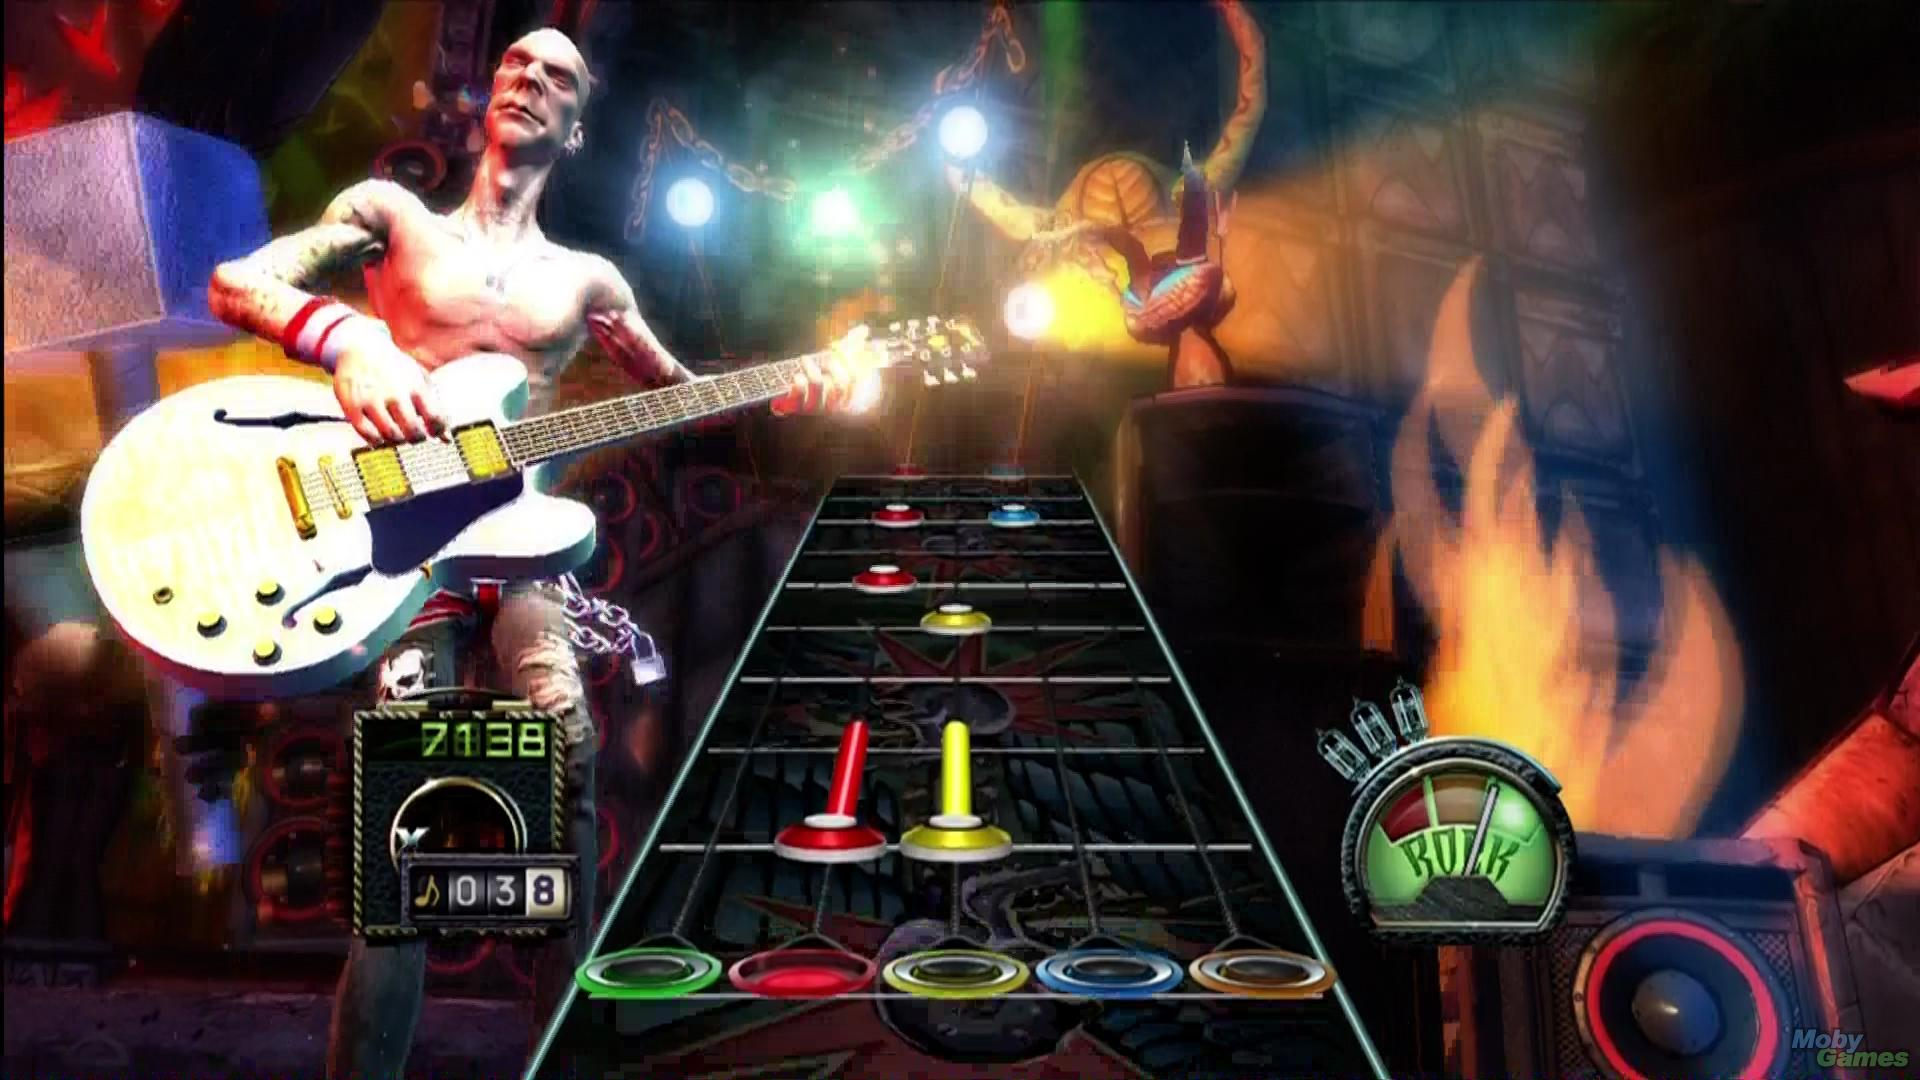
\includegraphics[width=0.7\linewidth]{figure/Analysis/guitarhero}
			\caption{Interactive music video game guitar hero.}
			\label{fig:guitarHero}
		\end{figure}
	\subsection{Noteput}
		German table where you physically put notes on it, and press play button to play notes, hopefully learning note and sheet theory.
	\subsection{Dato duo}
		Two person synthesizer for kids, no apparent learning outcome, but seems fun to play around with.
		\begin{figure}[H]
			\centering
			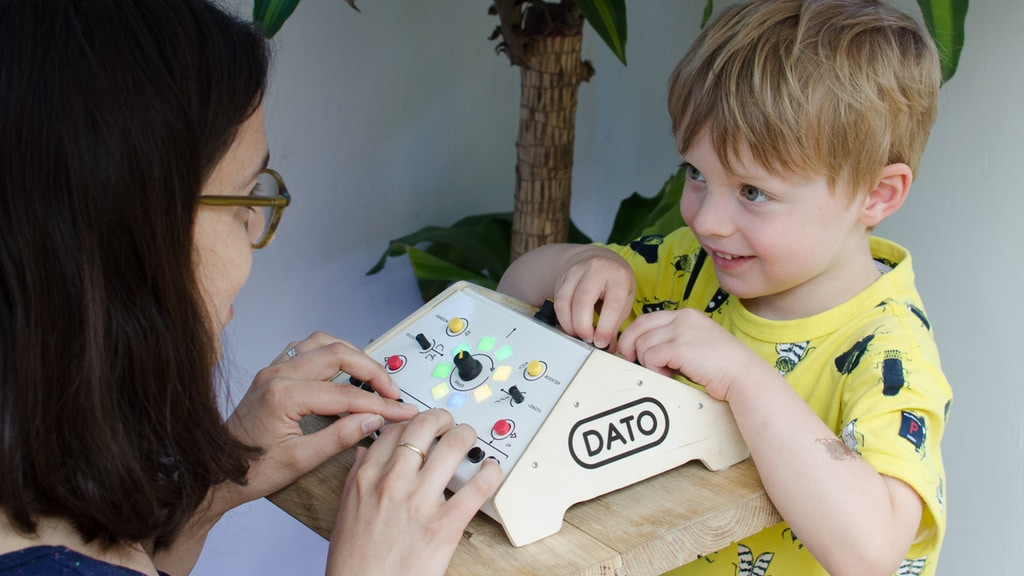
\includegraphics[width=0.7\linewidth]{figure/Analysis/datoduo}
			\label{fig:datoduo}
			\caption{Dato duo synthesizer}
		\end{figure}
	\subsection{Soundstage}
		VR application by Google, where you compose and play music in virtual reality. You can synthesize, plug things into other things, and create entire scores in this virtual reality playground.
		
	\subsection{V-Beat}
		The v-beat drumsticks are, for all its intents and purposes, simply air drumming.
		\begin{figure}[H]
			\centering
			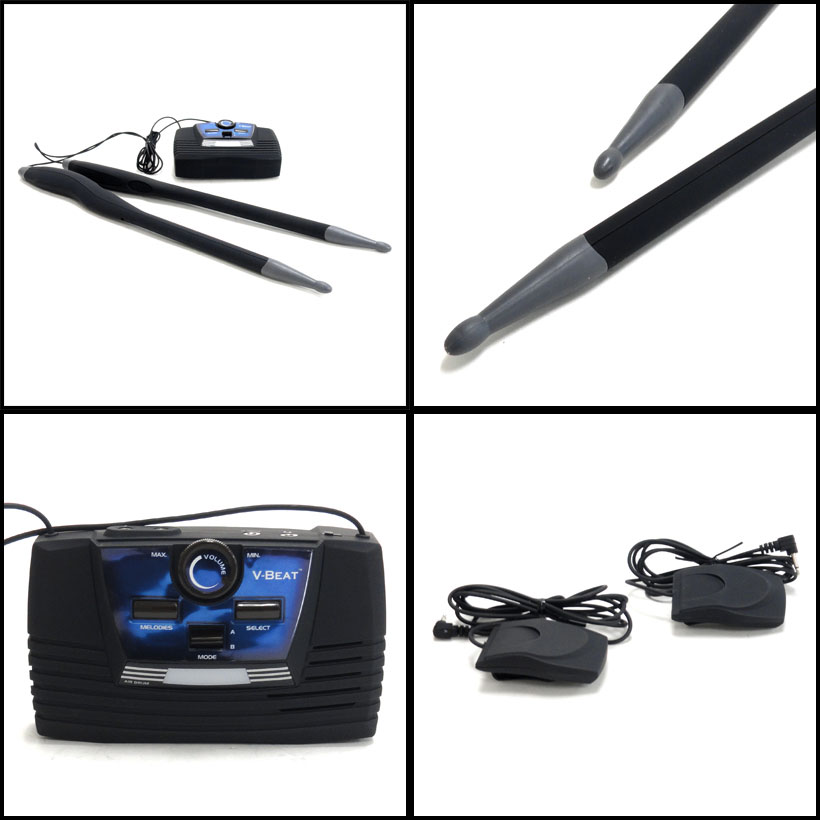
\includegraphics[width=0.5\linewidth]{figure/Analysis/vbeat}
			\label{fig:vbeat}
			\caption{Vbeat drumsticks}
		\end{figure}
		
	\subsection{MI Guitar}
		\begin{figure}[H]
			\centering
			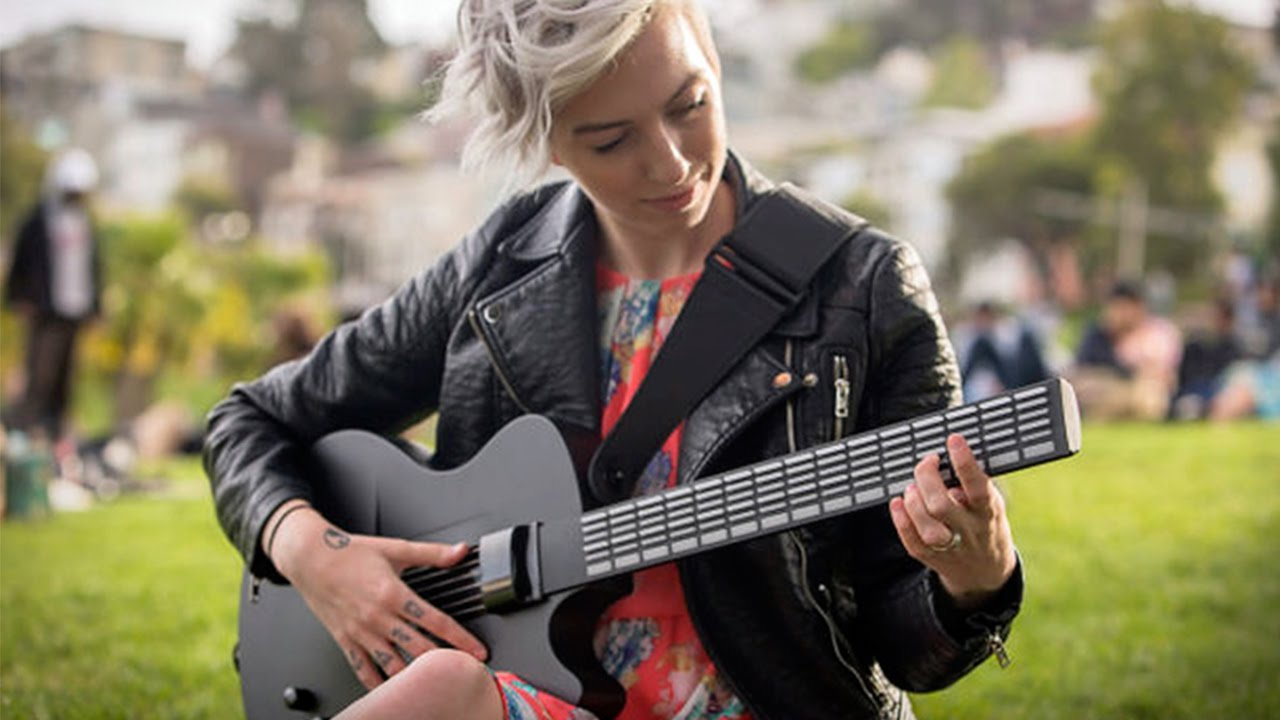
\includegraphics[width=0.8\linewidth]{figure/Analysis/miguitar}
			\label{fig:miguitar}
			\caption{MI guitar to teach guitar play}
		\end{figure}
	
	\subsection{Yousician}
		\begin{figure}[H]
			\centering
			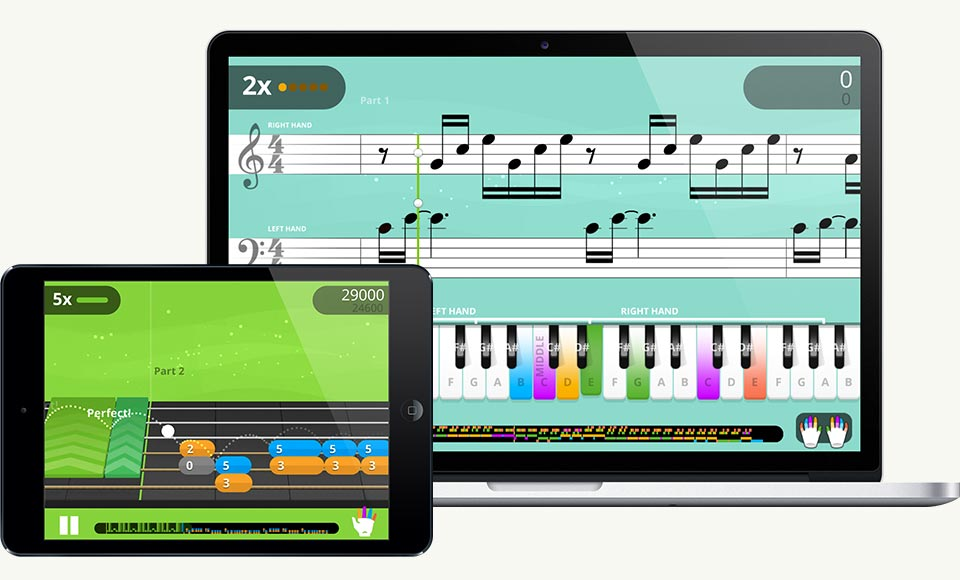
\includegraphics[width=0.8\linewidth]{figure/Analysis/yousician.jpg}
			\label{fig:yousician}
			\caption{Yousician}
		\end{figure}
	\subsection{Chrome Music Lab}
		\begin{figure}[H]
			\centering
			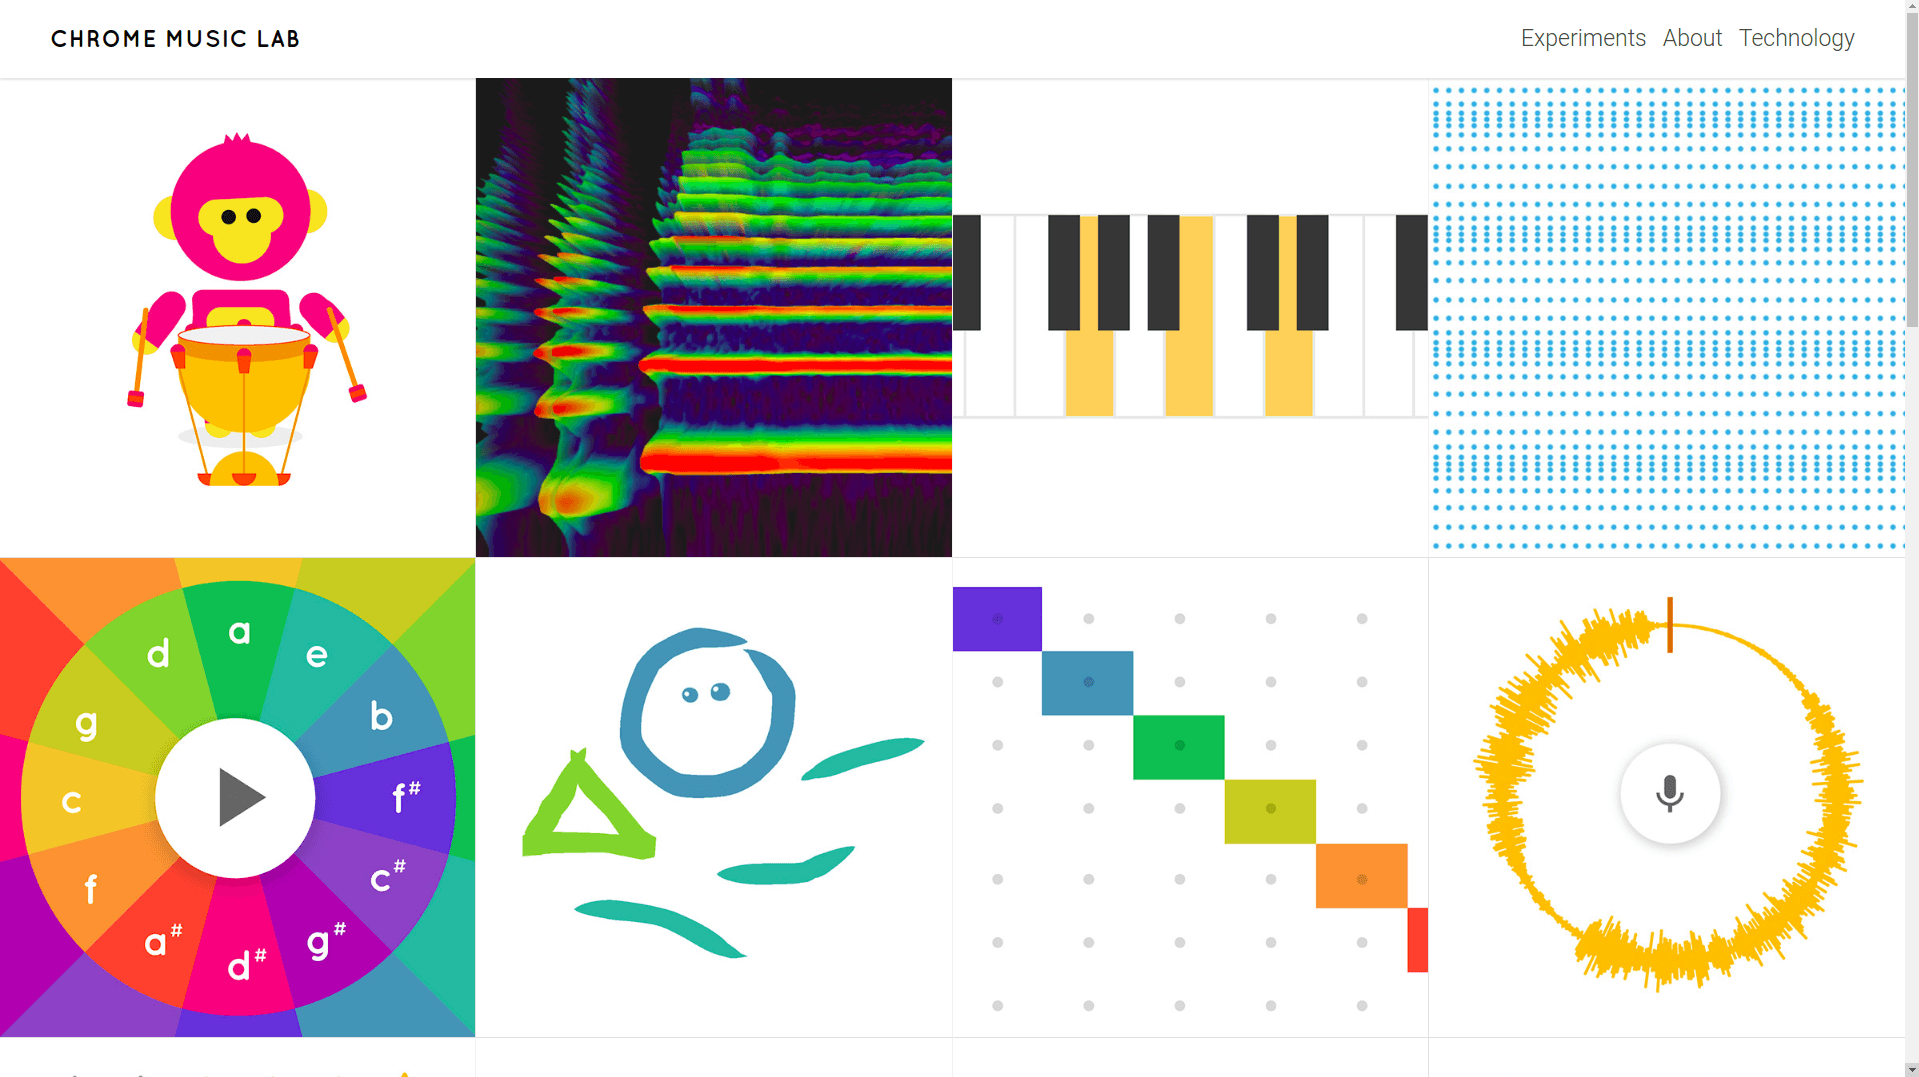
\includegraphics[width=0.8\linewidth]{figure/Analysis/chromeMusicLab.png}
			\label{fig:chromeMusicLab}
			\caption{Chrome Music Lab}
		\end{figure}

	\subsection{MuseScore}
	MuseScore is an open-source software program for creating music notation. The main attraction of the software is the ability to play and practise sheet music anywhere. You are able to search for new music sheets and practice thsese by either listening to the notes or change the notation. It is available for windows, mac, IOS, Android and Kindle Fire. It has an input via MIDI keyboard and can transfer to and from other programs via MusicXML, MIDI etc. This is a very useful tool for understanding music notation and practice it hands on. This software is a good example on learning notation for beginners to expert or just experts that want to create music. The program is build so that anyone wanting to create music can. MuseScore also provides their own definite guide to MuseScore. In contrast to many other softwares that lets one build notation sheets, this specific software is free. 
	\todo{This is one of the programs Hanna was talking about. Just wrote a little about it - we might not need to use it}
	
		\begin{figure}[H]
			\centering
			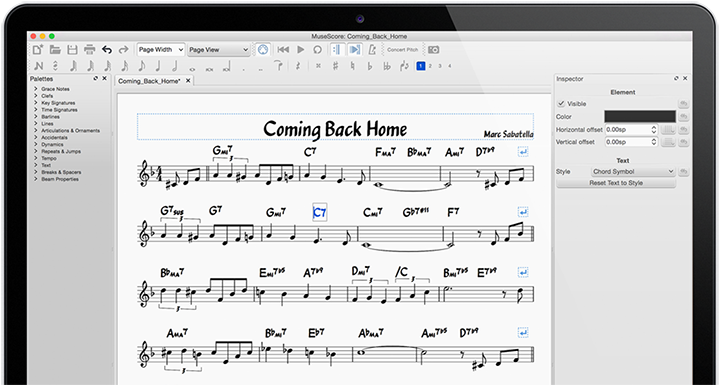
\includegraphics[width=0.8\linewidth]{figure/Analysis/musescore.png}
			\label{fig:MuseScore}
			\caption{MuseScore}
			\href{https://musescore.org/da}{\color{blue}here}
		\end{figure}
	
	
	
	
	
	
	
	
















		